\newpage
\section{Experiments}\label{sec:exp}
Our experiments are based on the timing performances of the three ILP techniques
we have used. We have set up our implementations in order to compare them in the
fairest way possible.\\
Table~\ref{tab:prf_cmp} offers an overview of the timings of the main tasks presented in Section~\ref{sec:impl}.
{\rowcolors{2}{gray!50!}{}
\begin{center}
    \begin{table}[h]
    \centering
    \begin{tabular}{ |l|c|c|c| } 
        \hline
        Task & \textbf{HYPER} & \textbf{Metagol} & \textbf{ILASP} \\ \hline
        \texttt{adjacent/2} & 175.884 & 0.056 & 4.767 \\ 
        \texttt{move/2} & 0.063 & 0.047 & 5.343 \\ 
        \texttt{move/2} (\(7*7\) grid) & 0.0716 & 0.054 & 5.432 \\
        \texttt{move/2} (\(9*9\) grid) & 0.0718 & 0.023 & 5.381 \\
        \texttt{reach/3} & 1.577 & 0.027 & NA \\ 
        \texttt{move/2} and \texttt{reach/3} & 7.077 & 0.848 & NA \\ 
        \hline
    \end{tabular}
    \caption{\label{tab:prf_cmp}Time comparison between the different systems for the main tasks (seconds)}
\end{table}
\end{center}
}
The timings show how the Maze dimension does not have an impact on the learning process (as for ILASP this is described
in another context at Section~\ref{sec:ilasp}).\\
The table also shows the similar behavior between HYPER and Metagol with regards of the \emph{combined
learning} of predicates \texttt{move/2} and \texttt{reach/3}. Both the implementations seem to
perform better in learning complex predicates when these are split in smaller tasks.
Comparing timings altogether, it is possible to notice how Metagol performs much better than the other
two systems. Given the similar approach between HYPER and Metagol, one could expect them
to also have similar performances. While HYPER uses a more general approach, Metagol owes its efficiency to metarules and the way they shape the language bias. This, though, does not come
for free, since defining good metarules requires a very accurate initial idea of what the final solution should be like.\\

Time performances were also measured to analyze the behavior of the systems with different quantities of examples offered.
For this experiment, we tested the implementations to learn the predicate \texttt{move/2} (\emph{learning to walk}) on more redundant examples than needed to check
whether this impacted time performances. The results of these experiment can be seen in Table~\ref{tab:ex_cmp}.

{\rowcolors{2}{gray!50!}{}
\begin{center}
    \begin{table}[h]
    \centering
    \begin{tabular}{ |l|c|c|c| } 
        \hline
        \(|E|\) & \textbf{HYPER} & \textbf{Metagol} & \textbf{ILASP} \\ \hline
        8 & 0.067 & 0.029 & 5.31 \\ 
        16 & 0.065 & 0.028 & 5.43 \\
        24 & 0.065 & 0.033 & 5.53 \\  
        \hline
    \end{tabular}
    \caption{\label{tab:ex_cmp}Time comparison with increasing examples (seconds)}
\end{table}
\end{center}
}
The timings show how the different quantities of examples used do not impact timing performances. This may not be true for way larger
quantities, for instance, Metagol would have to prove all those examples one at a time and, although this would be a trivial task,
with examples stacking up, it could start take a slightly considerable amount of time.

\subsection{Learning \texttt{reach/3} with \emph{tail recursion}}
Being \emph{"solving the Maze problem"} part of the title and one of the main goals of this project, we were
quite surprised that the \texttt{reach/3} predicate learned in our implementations was not able to find a path
in our Maze (Figure~\ref{fig:our}).\\
By studying the trace when querying Prolog with \texttt{reach((1,1), (2,5), L)},
we noticed that the search of the path would get stuck into a loop, going back and forth from cells \texttt{(5,2)} and
\texttt{(5,3)}. The reason of this behavior is related to the (partly) declarative nature of Prolog. The \texttt{reach/3}
predicate defined as in Listing~\ref{lst:res_rfsm} falls into a loop because, when getting at cell \texttt{(5,2)},
the predicate \texttt{reach\_2/2} is unified with the head of the first rule found in the program. Since there is
no \texttt{B} such that \texttt{inc\_x((5,2),B)}, Metagol will go for \texttt{dec\_y((5,2), B)}. This unification
will not work either since there is no \texttt{B} such that \texttt{dec\_y((5,2), B)} (\texttt{(5,1)} is an obstacle). At
last the unification is done with the rule at Line 5, with the body consisting to \texttt{inc\_y((5,2), B)} and hence moving
to cell \texttt{(5,3)}.\\
Now again, there is no \texttt{B} such that \texttt{inc\_x((5,3), B)}, so Metagol will unify the
\texttt{reach\_2/2} predicate with the head of the rule at Line 4, going for \texttt{dec\_y((5,3), B)} and, hence,
going back onto cell \texttt{(5,3)}.\\

In order to solve this issue we were able to \emph{"manually"} define a procedure for \texttt{reach/3} as shown in Listing~\ref{lst:r_tr}

\begin{figure}
    \centering
    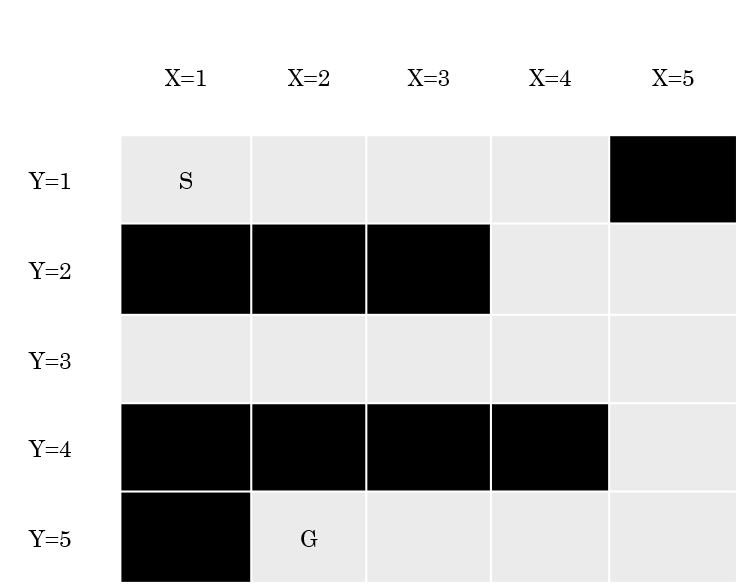
\includegraphics[scale=0.7]{img/ourMaze.png}
    \caption{The analyzed Maze}\label{fig:our}
\end{figure}

\begin{lstlisting}[label={lst:r_tr}, language=Prolog, caption=\texttt{reach/3} with tail recursion, belowcaptionskip=1cm]
reach(A,B,L) :- reach_1(A,B,[A],L).
reach_1(A,A,L,L).
reach_1(A,B,Acc,L) :-
    move(A,C),
    non_member(C,Acc),
    reach_1(C,B,[C|Acc],L). 
\end{lstlisting}
This procedure resembles the techniques for a loop preventing Depth-First Search. The idea behind this procedure is to store
the already visited cells into an accumulator (\texttt{Acc}) and, at each step, check whether a new encountered cell has already
been visited before.\\
Unfortunately, we were not able to learn this procedure through any of the mentioned ILP techniques.
\newpage